%% ============================================================
%% Revision Notes (2026-03-29, Yuyang):
%% 1. Core Principle: Already concise, kept as-is.
%% 2. Applications: Ensured each domain is one paragraph. Merged
%%    Fairness sub-themes (Cultural Adaptability + Demographic Fairness).
%%    Compressed Privacy into one paragraph. Cleaned up commented-out
%%    old versions of Safety and Factuality.
%% 3. Discussion: Removed from this file. Shortened version moved to
%%    sections/11-challenges_directions.tex with red source marker.
%% ============================================================

\subsection{Multi-Agent Systems}
\label{sec:multi_agent_systems}

\begin{figure}[htbp]
    \centering
    % Width uses \textwidth; height auto-scales with !
    \resizebox{\textwidth}{!}{%
        \begin{tikzpicture}

        % --- 1. Define leaf nodes (papers, citations added) ---
        \node[leaf] (safety_papers) {
            AutoDefense~\citep{zeng2024autodefense}, MARO~\citep{li2025multiagentframeworkautomateddecision}, PeerGuard~\citep{fan2025peerguarddefendingmultiagentsystems}, GUARDIAN~\citep{zhou2025guardiansafeguardingllmmultiagent}, Ebrahimi et al.~\citep{ebrahimi2025adversaryresistantmultiagentllmcredibility}, RedDebate~\citep{asad2025reddebatesaferresponsesmultiagent}, MASTER~\citep{zhu2025mastermultiagentsecurityexploration}, PsySafe~\citep{zhang-etal-2024-psysafe}, Qi et al.~\citep{qi2025amplifiedvulnerabilitiesstructuredjailbreak}, He et al.~\citep{he-etal-2025-red}.
        };
        \node[leaf, below=0.3cm of safety_papers] (factuality_papers) {
            Du et al.~\citep{10.5555/3692070.3692537, 10.5555/3692070.3693020}, CFMAD~\citep{conf/coling/0008L0HF25}, Markov-chain debate~\citep{10889448}, MAMM-REFINE~\citep{wan-etal-2025-mamm}, MADR~\citep{kim2024llmsproducefaithfulexplanations}, Audit-LLM (EMAD)~\citep{song2024auditllmmultiagentcollaborationlogbased}, CausalGPT~\citep{tang2025causalgptmultiagentapproachfaithful}, COOPERATE/COMPETE~\citep{feng-etal-2024-dont}, Collaborative Calibration~\citep{yang2024confidencecalibrationrationalizationllms}.
        };
        \node[leaf, below=0.3cm of factuality_papers] (fairness_papers) {
            Ki et al.~\citep{ki-etal-2025-multiple}, Mitigation via Selective Rewrite (MSR)~\citep{wan-chang-2025-white}, Multi-LLM (Owens et al.)~\citep{owens2024multi}, Borah \& Mihalcea~\citep{borah-mihalcea-2024-towards}, Wan et al.~\citep{wan2025culturallensmodelsadopt}.
        };
        \node[leaf, below=0.3cm of fairness_papers] (privacy_papers) {
            MASLEAK~\citep{wang2025ipleakageattackstargeting}, Li et al.~\citep{li-etal-2025-1}.
        };

        % --- 2. Define main sub-nodes (Trustworthiness dimensions) ---
        % Positioned to the left of corresponding leaf nodes
        \node[sub, left=0.5cm of safety_papers] (safety) {Safety};
        \node[sub, left=0.5cm of factuality_papers] (factuality) {Factuality \& Faithfulness};
        \node[sub, left=0.5cm of fairness_papers] (fairness) {Fairness};
        \node[sub, left=0.5cm of privacy_papers] (privacy) {Privacy};

        % --- 3. Define root node ---
        % Use the calc library to vertically center the root node relative to the sub-nodes
        \node[main, left=2.5cm of {$(safety.west)!0.5!(privacy.west)$}] (mas) {Multi-Agent Systems (§\ref{sec:multi_agent_systems})};

        % --- 4. Draw connection lines ---
        % a. Draw a main trunk from the root node to a branching point
        \coordinate (fork) at ($(mas.east) + (1.25cm,0)$);
        \draw[line] (mas.east) -- (fork);

        % b. Connect from main branching point to each sub-node
        \draw[line] (fork) |- (safety.west);
        \draw[line] (fork) |- (factuality.west);
        \draw[line] (fork) |- (fairness.west);
        \draw[line] (fork) |- (privacy.west);

        % c. Connect main sub-nodes directly to leaf nodes
        \draw[line] (safety.east) -- (safety_papers.west);
        \draw[line] (factuality.east) -- (factuality_papers.west);
        \draw[line] (fairness.east) -- (fairness_papers.west);
        \draw[line] (privacy.east) -- (privacy_papers.west);

        \end{tikzpicture}%
    }
    \caption{A taxonomy of Multi-Agent Systems for enhancing LLM trustworthiness.}
    \label{fig:mas_taxonomy}
\end{figure}

Multi-Agent Systems (MAS) represents a fundamental paradigm shift in controlling LLM behavior. Instead of focusing on a single, monolithic model, this approach architects a system of multiple, interacting LLM-based agents. Within this framework, trustworthiness is not a property enforced upon a single model but rather an emergent property of the system's collaborative dynamics. By structuring interactions through mechanisms such as debate, adversarial simulation, and multi-perspective deliberation, MAS can achieve levels of robustness, safety, and factuality that are often unattainable by individual agents.

\subsubsection{Core Principle: From Monolithic Control to Collaborative Systems}

The core principle of multi-agent systems is the decentralization of reasoning and decision-making. A complex problem is decomposed and assigned to specialized agents, each potentially embodying a unique role, persona, or expertise. Trustworthiness is fostered through the design of their interaction protocols, which can include adversarial debate, cooperative problem-solving, peer review, or hierarchical verification. For instance, a ``propose'' agent might generate an initial response, a ``critic'' agent might challenge its assumptions and check for flaws, and a ``synthesize'' agent might integrate the feedback to produce a final, more considered output. This structured interaction creates an intrinsic error-correction and validation mechanism at inference time. The system's reliability, therefore, depends less on the perfection of any single agent and more on the robustness of the collaborative architecture itself.


\begin{figure*}[htbp]
  \centering
  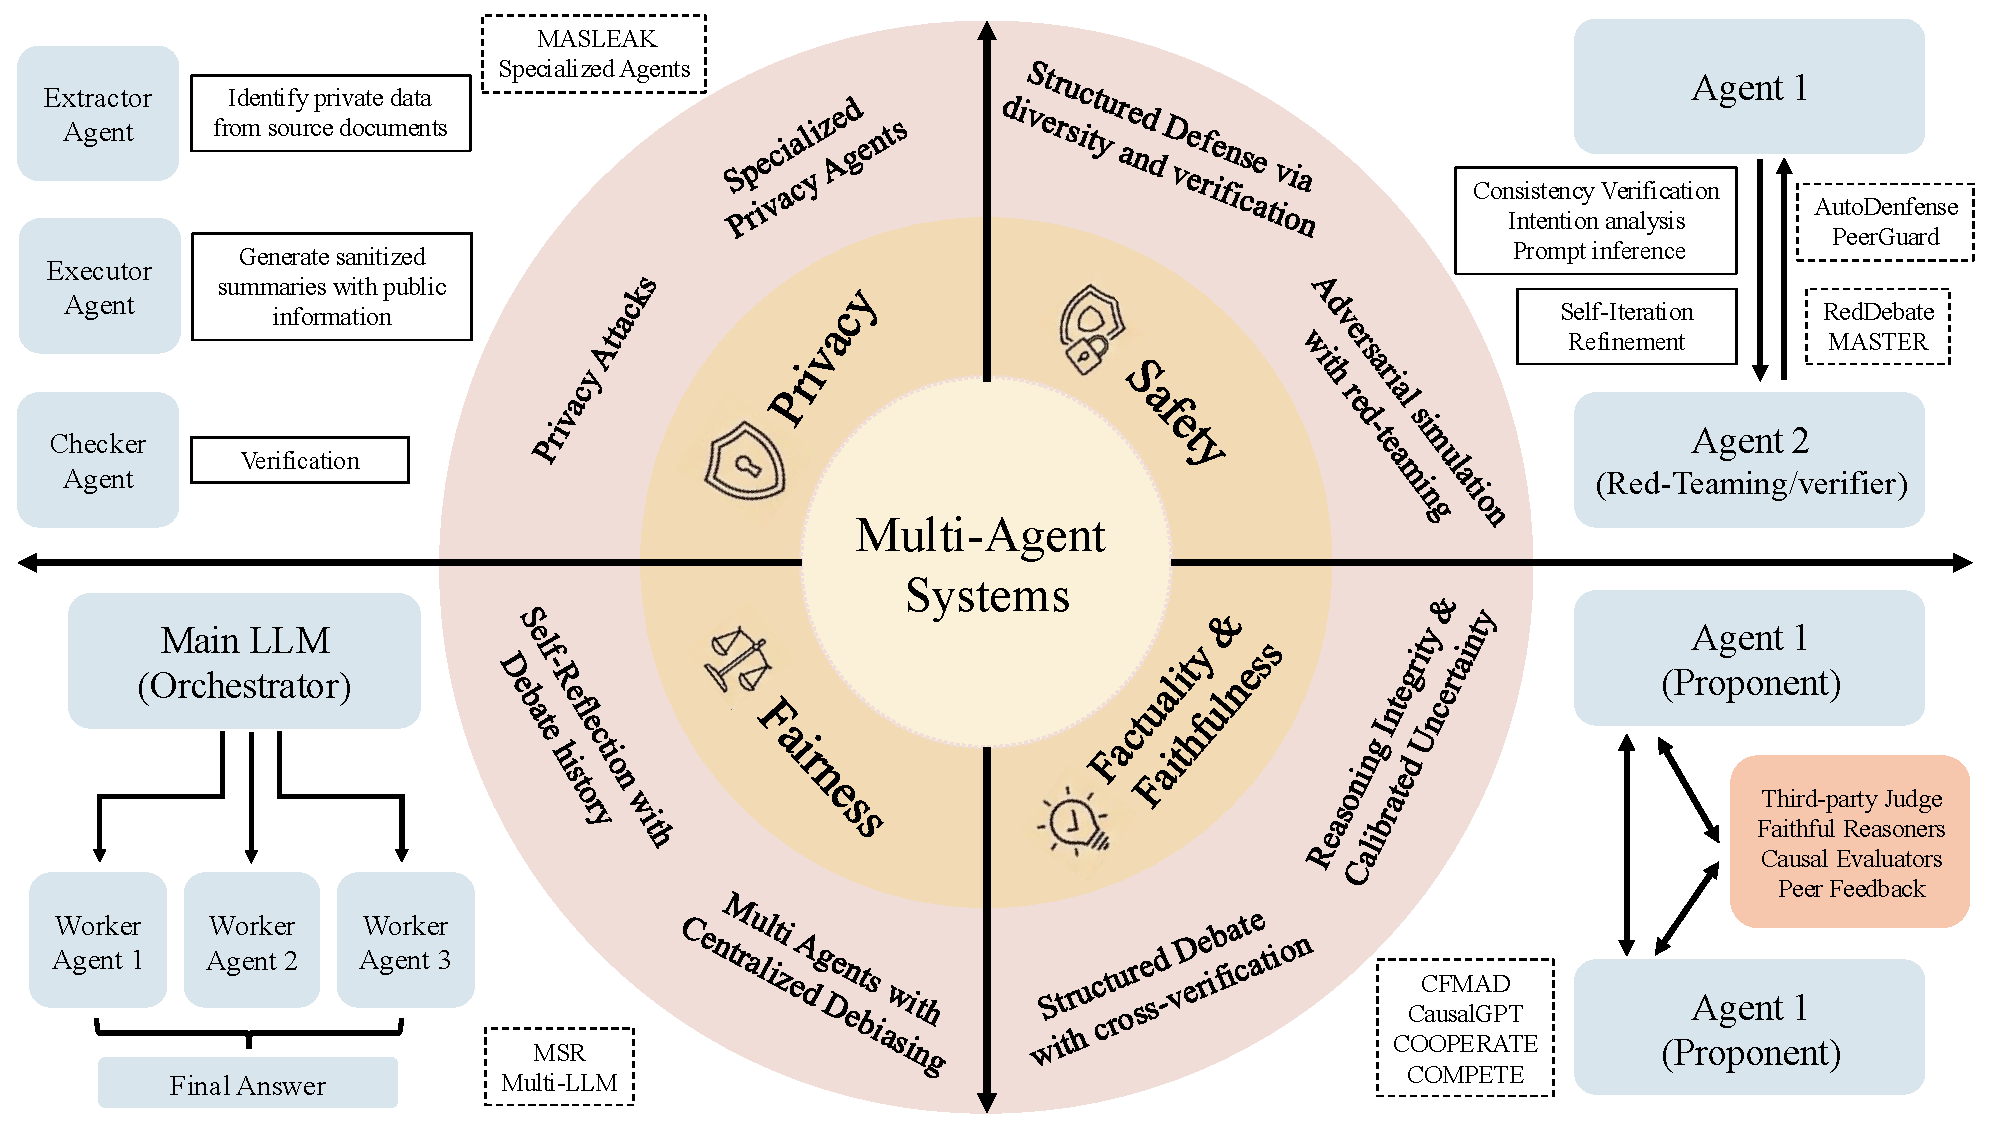
\includegraphics[width=0.9\linewidth]{figures/method/multi_agent.pdf}
  \caption{Overview of multi-agent system architectures for LLM trustworthiness across four dimensions. Safety employs structured defense via role diversity and adversarial red-teaming; Factuality relies on structured debate with cross-verification and calibrated uncertainty; Fairness uses multi-agent debiasing with self-reflection as well as orchestrated plan-and-refine loops; and Privacy leverages specialized agents (Extractor, Executor, Checker) for data sanitization. Representative systems and interaction patterns are shown for each dimension.}
  \label{fig:method_multiagent}
\end{figure*}

\subsubsection{Applications}
\paragraph{Safety}

Multi-agent systems turn safety from a static, single-model property into an emergent outcome of \emph{structured interaction}. Instead of relying on one model's filter, MAS instantiate a propose--attack--audit--adjudicate loop: specialized agents generate responses, probe for failures, cross-check reasoning, and arbitrate outcomes. A unifying pattern is \emph{structured defense via role diversity and cross-verification}. Systems like AutoDefense orchestrate intention analysis, prompt inference, and final judgment to filter unsafe outputs~\citep{zeng2024autodefense}. Committee-style analyzers extend coverage by combining linguistic, comment, and fact-checking expertise for misinformation risks~\citep{li2025multiagentframeworkautomateddecision}. Peer-based scrutiny hardens internal logic: PeerGuard has agents verify consistency between each other's chain-of-thought and final outputs to expose backdoors~\citep{fan2025peerguarddefendingmultiagentsystems}. At system scale, collaboration can be modeled as a temporal interaction graph to trace and arrest the spread of hallucinations or injected errors~\citep{zhou2025guardiansafeguardingllmmultiagent}, and dynamic credibility weighting further down-ranks unreliable contributors~\citep{ebrahimi2025adversaryresistantmultiagentllmcredibility}. Safety also benefits from \emph{adversarial simulation for proactive discovery}: automated red-teaming with debate has agents iteratively elicit, refine, and then patch unsafe behaviors using persistent memory~\citep{asad2025reddebatesaferresponsesmultiagent}. However, the same interactive channels expand the attack surface---structured debates can amplify jailbreak success~\citep{qi2025amplifiedvulnerabilitiesstructuredjailbreak}, communication links invite Agent-in-the-Middle manipulation~\citep{he-etal-2025-red}, persuasive agents can steer group consensus toward unsafe actions~\citep{zhang-etal-2024-psysafe}, and comprehensive security taxonomies such as MASTER map these vulnerabilities~\citep{zhu2025mastermultiagentsecurityexploration}, and broader analyses of \emph{emergent social risks} reveal how misaligned agent interactions can produce system-level harms that no individual agent was designed to cause~\citep{huang2026emergent}.

\paragraph{Factuality}

Multi-agent systems enhance factuality and faithfulness by replacing a single model's unverified reasoning with structured interaction among diverse agents. Rather than trusting one model's first-pass answer, MAS organize a propose--critique--adjudicate loop in which agents advance claims, attack each other's reasoning, and converge under a judge. Foundational work shows that debating agents can reach more accurate conclusions than individuals, as critiques expose faulty logic that a single model may miss~\citep{10.5555/3692070.3692537}, and debates judged by weaker raters still tend to favor truthful arguments~\citep{10.5555/3692070.3693020}. Forced-disagreement variants such as CFMAD assign counterfactual stances to improve robustness to initial mistakes~\citep{conf/coling/0008L0HF25}. This pattern scales to long-form tasks by decomposing outputs into atomic claims and verifying each through coordinated agents, including role-structured stateful debates~\citep{10889448}, discriminative reranking pipelines~\citep{wan-etal-2025-mamm}, complementary-perspective feedback for explanation faithfulness~\citep{kim2024llmsproducefaithfulexplanations}, and domain-specific evidence cross-examination~\citep{song2024auditllmmultiagentcollaborationlogbased}. Beyond surface correctness, MAS can promote reasoning integrity through separating faithful reasoners from causal evaluators~\citep{tang2025causalgptmultiagentapproachfaithful}, and calibrated uncertainty through peer feedback and adversarially generated alternatives that reveal knowledge gaps and trigger abstention~\citep{feng-etal-2024-dont, yang2024confidencecalibrationrationalizationllms}.

\paragraph{Fairness}
Multi-agent systems offer a promising path toward adaptively resolving complex biases across generation tasks, addressing demographic biases embedded in language patterns that simpler mitigation methods cannot effectively handle. A key direction is leveraging multi-agent debate to improve cultural adaptability:~\citet{ki-etal-2025-multiple} propose a framework where multiple LLM agents approach culturally situated questions through a mixture of debate and self-reflection actions, with a judge LLM resolving disagreements based on debate history. For demographic fairness, multi-agent architectures decompose the debiasing task across specialized roles: Mitigation via Selective Rewrite uses an LLM agent to provide targeted feedback on removing gender bias in language style~\citep{wan-chang-2025-white}, multi-LLM frameworks incorporate multiple models in conversational settings with both centralized and decentralized debiasing configurations~\citep{owens2024multi}, and self-reflection mechanisms enable models to identify and self-correct societal biases through a critique step~\citep{borah-mihalcea-2024-towards}.
Most recently, ~\citet{wan2025culturallensmodelsadopt} proposes an agentic planning pipeline with high autonomy, which orchestrates an iterated diagnose-and-refine loop until model generation reaches a satisfactory state.

\paragraph{Privacy}

While multi-agent systems introduce powerful mechanisms for safety and factuality, they also create novel privacy challenges representing a significant research gap. The interconnected nature of MAS establishes new vectors for data leakage: the MASLEAK framework demonstrates systematic, worm-like attacks that can extract high-value intellectual property such as system prompts, tool definitions, and topological structure from black-box MAS applications by propagating through agent communication chains~\citep{wang2025ipleakageattackstargeting}. Conversely, the same architectural principles can be leveraged for defense: multi-agent approaches decompose the complex task of privacy preservation into specialized roles---such as an Extractor Agent to identify private data, an Executor Agent to generate sanitized outputs, and a Checker Agent for verification---significantly reducing leakage of sensitive information while preserving output quality~\citep{li-etal-2025-1}. These studies highlight a critical duality where the collaborative structure of MAS is both a liability and an asset for privacy, though a holistic understanding encompassing robust defenses, secure communication protocols, and verifiable information-flow controls remains largely unexplored.
